\section{はじめに}

ギリシャといえば今や国家の財政破綻や中近東の難民の大波ばかりが目立つ状態
ですが, ギリシャから我々はさまざまな恩恵を我々は受けています. 怪しいもの
ではBLとGLの同性愛, 重要なものでは神話, 詩や悲劇, 彫像や建築, 哲学や論理学
\footnote{論理学を発明・発展させた民族は他にインド人しかいないのです.
 中国戦国時代の墨家にも「墨子」\cite{墨子}から三段論法らしき推論を含む論理学
があったことが伺えますが残念なことに途絶えています.}, 数学や天文学に医術等
の科学全般でしょうか.
\newline

BLでは古代ギリシャの都市国家テーバイ(\textgreek{J'hbai})の
「\textbf{神聖隊(\textgreek{>Ier'o L'oqos})}」
\footnote{某アイドルグループとその所属事務所に傾向等が似ていても違います.}
を語らずにはいられません. この神聖隊は名前だけでは
「\textbf{やおいのか硬いのか判らない}」のですが, 実際は
「\textbf{とてもやおく}」て「\textbf{とても硬い}」のです. まず
「\textbf{やおい}」ことについて語るなら, 神聖隊は恋人達(当然, 男)
150組, 300名で編成されており, 「\textbf{硬さ}」について語るなら, 彼等は
「\textbf{精鋭歩兵部隊}」だったのです.
\newline
 
 
\begin{wrapfigure}{l}{5cm}
\includegraphics[width=5cm]{arno_breker_kameradschaft.pdf}
\caption{ブレーカー:戦友}
\label{fig:breker2}
\end{wrapfigure}

この部隊を編成した理由が, 恋人に無様な自分を見せたり危険な目に合わせ
る訳にも行かないがために勇敢に戦うだろうとかで, 実際, テーバイをギリシャ
の覇権国家にする要因の一つになったと云います.
\newline

ところで神聖隊はマケドニア王国とギリシャの覇権を巡ってカロネイアの戦いで
王太子時代のアレクサンダー大王(\textgreek{>Al'exandros G'})率いる騎兵隊
とマケドニア式ファランクス(\textgreek{f'alanx})のために254名
(ぴったり偶数!)が討死するという壊滅的打撃を受けます. マケドニア王
ピリッポス2世(\textgreek{F'ilippos B'})は彼等の亡骸を見て涙したとのこと
ですが, 戦いの半ば以降は図\ref{fig:breker2}の有様でしょうか. ちなみに
これはナチス時代の人気彫刻家ブレーカー(Breker)\footnote{ブレーカーの
戦時中の手記\cite{ブレーカー}が出版されていますが, その内容は非常に
まともです.}のレリーフで, この味わいも現実の突撃隊の同性愛を含む酒池肉林
に変幻するというものでしょうか? たとえば図\ref{fig:rrevue}のように...

\begin{figure}[htbp]
\begin{center}
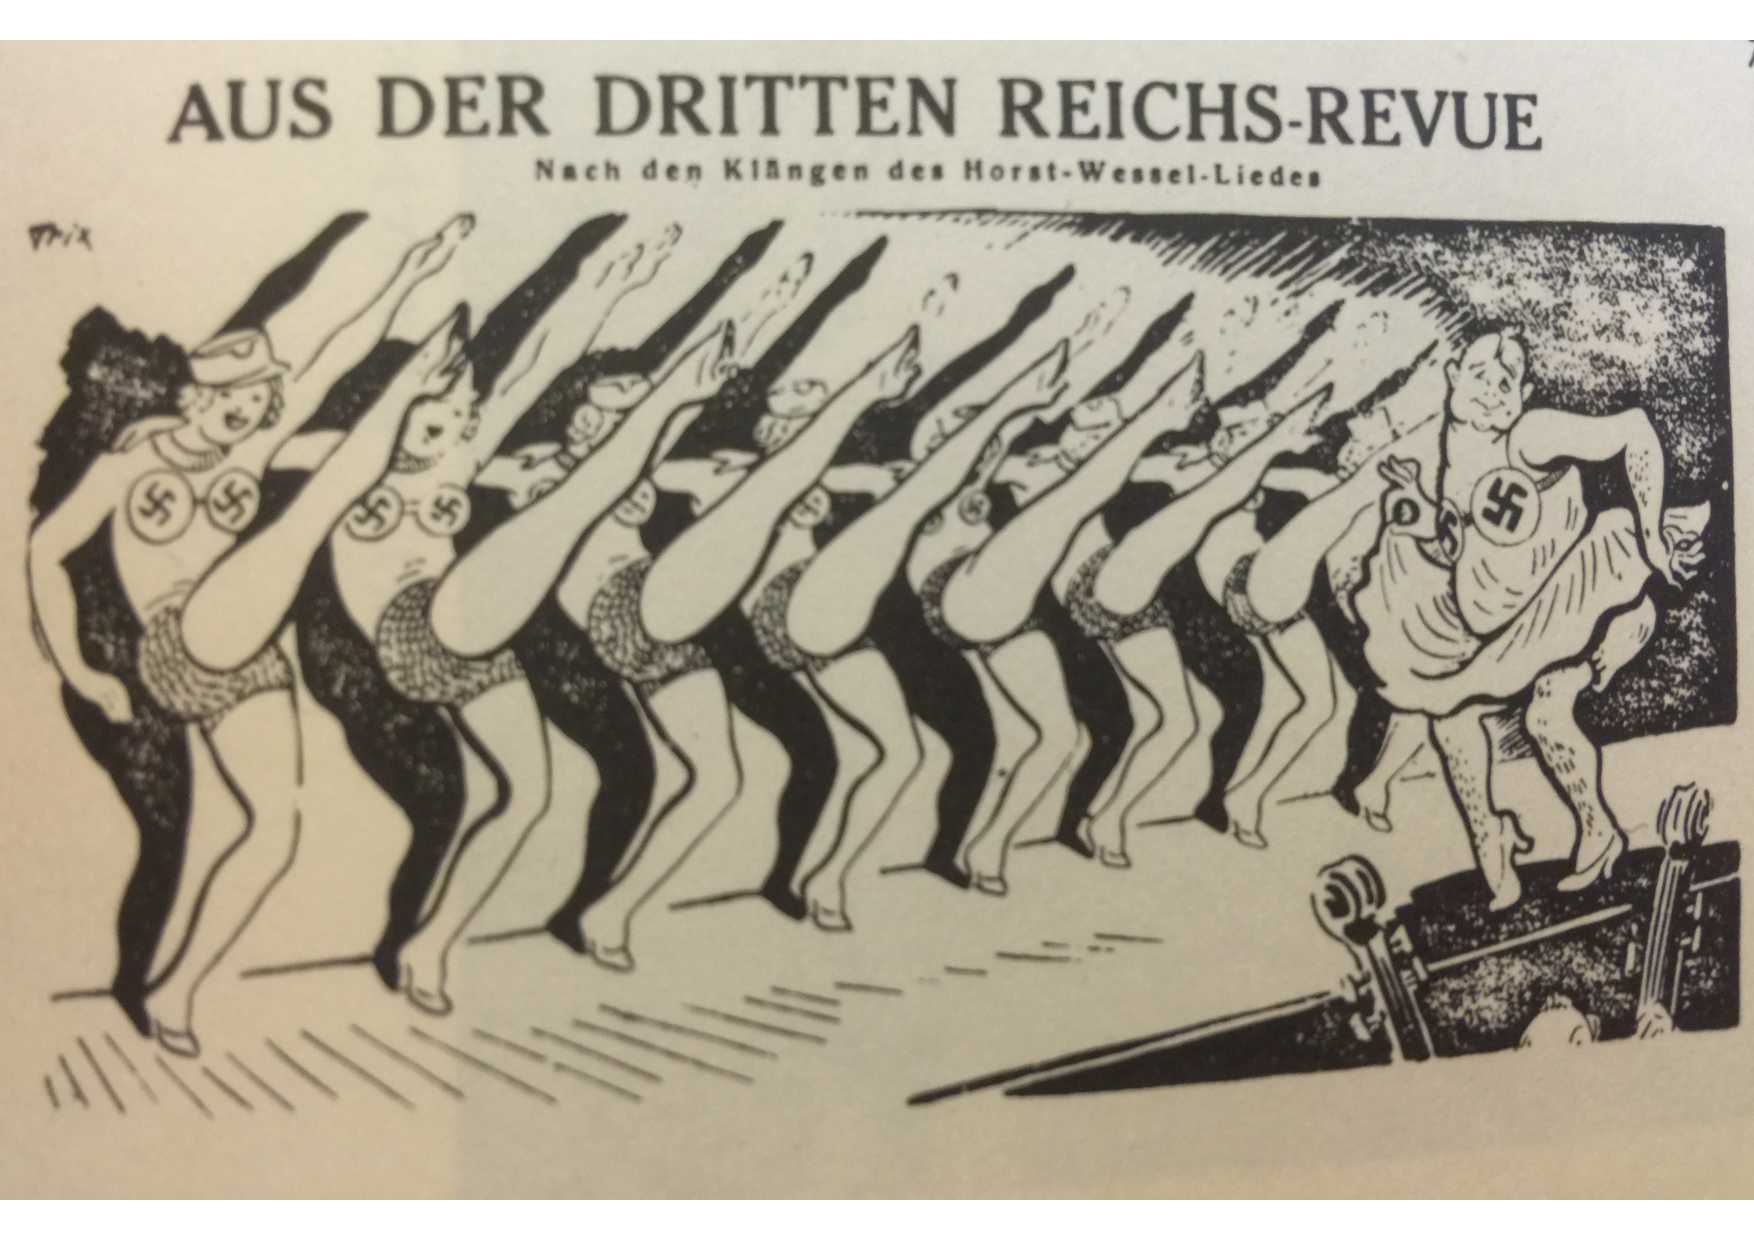
\includegraphics[width=8cm]{DrittenReichsRevue.pdf}
\caption{第三帝国のレビューより\cite{関}}
\label{fig:rrevue}
\end{center}
\end{figure}

ここで茶化されている人物は突撃隊幕僚長のレーム(R\"ohm)です. 彼はナチス
(NSDAP)の古参党員の一人でヒトラー(Hitler)の友人でした. ところが彼は
乱暴者, 男色家としても著名で, 「\textbf{私のところにいる男たちは法律に
反した特別なことに慣れねばならない}」と豪語し, 彼が在任中の突撃隊で同性愛
が横行したといいます. さらに彼は「国家社会主義」の「社会主義」に重点を
置いて「第二革命」を主張し, 突撃隊の国軍化を図ったことから国防軍に警戒
され, 親衛隊によって「長いナイフの夜」で粛清されてしまいます. この粛清
ではナチス左派が粛清され, 粛清以降は同性愛は徹底的に禁じられます
\footnote{「ドイツ第三帝国」\cite{クラーザー}が文化的な側面にも言及が
あり良い本です. また, ジョークについては「ヒトラー・ジョーク」\cite{関}
が決定版でしょう. この本からヴィスコンティ(Visconti)の「地獄に堕ちた
勇者ども(The Damned)」が連想される図\ref{fig:rrevue}を選びました.}
\newpage

\begin{wrapfigure}{l}{5cm}
\includegraphics[width=6cm]{Breker2_relief.pdf}
\caption{ブレーカー:戦士の出発}
\label{fig:breker1}
\end{wrapfigure}

ここでナチス公認芸術は図\ref{fig:breker2}のような何はともあれ一応英雄的
なものや図\ref{fig:breker1}のように何だかよく判らないけどカッコエー代物
(裸体にマントがス・テ・キ$\heartsuit$)だとか, まあ随分と同性愛一歩手前
のきわどいものだったのです\footnote{女性絵画になると... ちなみに女性画
の公認巨匠ツィーグラー(Ziegler)は「\textbf{ドイツ恥毛の巨匠}」と呼ばれ
ていたそうです. それに苦言を呈する党員も居たそうですが「\textbf{兵士達
は美しいものに飢えているんだ!}」の一言で片付けられたとか.}. こういった
胡散臭い代物でも, 男の私でもある種の「憧憬」を感じてしまうのです. 実際,
 こんな偉丈夫に「\textbf{俺に付いて来い!}」と壁ドンされるとどうですか?
 「\textbf{うほ!?}」とならないにせよ「\textbf{面白い冒険が始まりそう..}」
と思ってフラフラと付いて行く男も多いのではないでしょうか?
 ただ, 古代ギリシャの同性愛は性的なもの以上に「\textbf{若者は年長者の
名声と知恵に憧れ, 年長者は若者の若さと美に憧れる}」という至って素朴な
ものだったのではないかと私は思っています.
\newline

さて, ナチスはギリシャ文明を「\textbf{北方化}」したくて仕方なかったようです.
 実際, 北方からドーリア人(\textgreek{Dwrie'is})等の侵入がミケーネ文明崩壊
の原因の一つとされ, スパルタ(\textgreek{Spart'a})は先住民を征服してとんでも
ない占領政策を続けているのでそう言いたくなるのも判らない訳でもありません.
 これもゲーテ(G\"othe)が悲劇ファウスト(Faust)\cite{ゲーテ}で, 元ネタの人形劇
ファウストにて絶世の美人の例でしかなかったヘレネー(\textgreek{<El'enh})に
ヘレニズム文明を体現させてドイツ・バロック的なファウストと結婚させることで
自らの古典主義を賛美したあたりからでしょか\footnote{ヘレネー:「私はひどく
遠くにいるような, そのくせ近くにいるような気がします..」\cite{ゲーテ}
第二部, 第三幕}?  ゲーテはさておきその亜流連中にとってはフランスがラテン
文化の後継者なら, ドイツはより源流のギリシャ文明を取るといった安易な
民族主義が根幹にあったのかもしれません. なお, 野蛮なゲルマニアをそのまま
受け入れるようになったのはロマン主義も後期に入ってからのことです
\footnote{当時のお隣のロシア帝国も同様で, 19世紀のチャイコフスキー
({\cyr{Cha{\u i}kovski{\u i}}})のバレエは主に中世ドイツの宮廷や
フランス的な貴族の館の話ですが, 20世紀初頭のプロコフィエフ
({\cyr{Prokof{\cprime}ev}})やストラビンスキー({\cyr{Stravinski{\u i}}})
になるとスキタイ人や古代ロシア人, でなければ民話といったあんばいです.
 では日本は? 政治的風潮で軍国主義を高貴と讃え, 米英を卑しい商人の国と
軽蔑したのが第一次世界大戦中のドイツ\cite{クラウス}, 日本ではそれを
1930年代後半と20年近く遅れています.}.
\newline

ともあれナチスについて言えば, 普遍性に背を向けて19世紀末の夜郎自大的
民族主義にどっぷり染まり, ワーグナー(Wagner)のオペラの絢爛豪華さに感激
した「\textbf{永遠の半端者共}」, 2ちゃん用語の「\textbf{厨房共}」で,
 「\textbf{聖なる愚か者}」のジークフリート(Siegfried)を
「\textbf{金髪の野蛮人}」に単純化して彼等の青少年を染め上げた結果,
 のちにギリシャ文明の担い手になったドーリア人どころか西ローマ帝国を
崩壊させて暗黒時代を招来したヴァンダル族(Vandal)以上の想像を絶する惨禍
を招いてしまったのです. 19世紀初頭のドイツはヘルダーリン
(H\"olderlin)によれば「\textbf{人がいるが人間がいない! ドイツ人ほど
支離滅裂な国民はいない. 職人はいる, だが人間がいない. 思想家はいる,
 だが人間がいない. 牧師はいる, だが人間がいない.}」と嘆く有様で,
 この状況はのちの哲学者ニーチェ(Nietzsche)にとっても同様で
「ツァラトゥストラはこう言った」で 「\textbf{耳が肥大化した人間}」等
の戯画化で「\textbf{専門バカ}」や「\textbf{教養主義の俗物}」を揶揄
しているのです(\cite{ツァラトゥストラ},救済)\footnote{ヘルダーリン
のそれは「ヒューペリオン」で失意の主人公がドイツに行ったときの感想です.
 ニーチェがそれを受けていることは「\textbf{戦場か屠殺場のように}」
 とヒューペリオンと同じ表現があることで判ります.}.
\newline

ところでニーチェの著作「悲劇の誕生」\cite{悲劇の誕生}を読むと猛烈な古代
ギリシャへの憧れが見受けられます. この「悲劇の誕生」では
「ディオニューソス(\textgreek{Di'onusos})」的なるもの, すなわち,
情念と「アポローン(\textgreek{>Ap'ollwn})」的なるもの, すなわち,
 理念の対峙を取り挙げた論文で, ワーグナーの楽劇をよいしょするものでも
あったために「\textbf{未来の文献学}」\footnote{ニーチェの本来の専門
は文献学で, ワーグナーは自分の音楽のことを「\textbf{未来の音楽}」と
呼んでいたことへの当て付けです.}と皮肉られています. その結びの一節に
「\textbf{美がこのように絶えず押し寄せてくる時...}」とありますが,
 実に古代ギリシャは偉大なのです. ところが我々日本人は残念なことに
近代化の時点で目覚しく発展しつつあるプロシア=ドイツ帝国に目を奪われ,
 その結果, ドイツ好きは沢山居ても, 西洋文明の源泉たるギリシャへの関心
が斯くも少ないのが現状なのです\footnote{文学では「潮騒」の三島由紀夫
でしょうか.}. そしてこの駄文の目標はギリシャ哲学と計算機科学を強引に
結び付けようとする分不相応な企てなのです. 時代を越えてファウストが
ヘレナに憧れ, 彼女と共にアルカディア(\textgreek{>Arkad'ia})にあらんと
するように私もそれを目指すのです.

\section{プラトンのイデア論}


主題の「\textbf{オブジェクト指向プログラミング(Object Oriented
 Programing)}」ですが, これはオブジェクトという概念を導入することで
プログラミングの生産性向上を図っていると説明されます. 具体的には, クラス
というオブジェクトの雛形を用意し, その雛形を使ってプログラムが扱うデータ
に対応するインスタンスを生成して処理を行うこと, クラスには属性やメソッド
があり, インスタンスの処理でそれらが使えること, クラス間に親子関係に類似
した階層構造があり, 属性やメソッドが継承と呼ばれる手続で下位のクラスの
インスタンスでも使えるという長所があることでしょうか.
\newline

このオブジェクトがクラスから創られる様子を説明するために古代ギリシャの
哲学者プラトン(\textgreek{Pl'atwn}, Plato)の「\textbf{イデア論(Theory
 of Forms)}」が引っ張り出されることがあります. このイデア論によれば
我々が考察の対象とする「\textbf{個体(individual)}」には
「\textbf{思惟によってのみ知られる世界}」, すなわち「\textbf{イデア界}」
に「\textbf{イデア(\textgreek{>id'ea}, idea)}」が存在し, 個体は
そのイデアの像であるというものです. だから貴方のそばに居る三毛猫の
「\textbf{みけ}」には対応する「\textbf{三毛猫のイデア}」が
「\textbf{イデア界}」に存在し, そのイデアの現世での像が
「\textbf{みけ}」であるという主張です. そしてイデアは思惟によってのみ
知覚できることに加え, さらには「\textbf{永遠不滅}」といった超越的な
性質を持っています. このことからイデアは現実にある対象を
「\textbf{理想化したもの}」で, ちょうど「\textbf{鋳型}」のような役割を
していると言えるでしょう. ただし, プラトンはイデア界こそが真実の世界で,
 現世はイデアが投影された「影の世界」, つまり
「\textbf{模倣物(\textgreek{e>ik'wn})の世界}」と考えています
(「洞窟の比喩」\cite{国家}). ここでオブジェクトが計算機上のデータとして
「\textbf{実体化}」することを「\textbf{インスタンス化(instantiation)}」, 
「\textbf{実体化したオブジェクト}」のことを
「\textbf{インスタンス(instance)}」と呼びますが, 
「\textbf{イデアの現世における実体化}」も英語では同じ
「\textbf{instantiation}」です. と, このようにクラスとインスタンスの
関係はイデアと実物との関係に類似しています. 
\newline

さて, 誰がイデアを実体化し, 理由が何であるかという素朴な疑問に対して,
 プラトンは歯切れが悪くなります. まず実体化させたのは
 「\textbf{デーミウールゴス(\textgreek{dhmiourg'os})}」で, イデアを
模倣して世界を創世した理由は貧欲な神「\textbf{エロース(\textgreek{>'Erws})}」
がイデアの美に憧れたからと述べていますが, 簡単に納得できるものでは
ありません. また, イデアは美や善に関わるもので醜いものや悪にイデアは存在
しないとも述べていますが, 「\textbf{何が美なのかをヒキガエルに聞いてみろ!}」
とヴォルテール(Voltaire)ならずとも言いたくもなるでしょう.
\newline


このような「\textbf{機械仕掛けの神(Deus ex machina)}」\footnote{
古代ギリシャ悲劇で収拾がつかなくなった話を解決するために唐突に神を登場
させる手法(ソフォクレース(\textgreek{Sofokl'hs})の
「ピロクテーテース(\textgreek{Filokt'hths})」のヘーラクレース
(\textgreek{<Hraklhs}))のことです.}を持ち出されても信じるしかない点は哲学
というよりも宗教です. 実際, ヘレニズム文明では, このイデア論を基に超越的な
「\textbf{一者(\textgreek{to >'en}, to hen)}」からの流出による世界の創造
(流出説)を取り入れた「\textbf{新プラトン主義}」\footnote{後世の呼び名で,
 御当人達はプラトンの思想と一致していると思っています.}, デーミウールゴス
による悪しき世界の創造, 不死でありながら肉体に囚われた人間, そして死後の
超越的な神への帰一を柱とする「\textbf{グノーシス主義(\textgreek{Gnwsis})}」
へと繋がります.


\begin{wrapfigure}{l}{4cm}
\includegraphics[width=4cm]{HermesTrismegistusCauc.pdf}
\caption{ヘルメス・トリスメギストス}
\label{fig:trismegistus}
\end{wrapfigure}

このグノーシス主義の文献に「 ヘルメス・トリスメギストス(三重に偉大な
ヘルメス, Hermes Trismegistus, \textgreek{<Erm\~es Trism'egistos})
が記したとされた\textbf{ヘルメス文書}」と呼ばれる一連の文書があります.
 ここでのヘルメスはギリシャ神話の神ヘルメスとエジプト神話の神トートが
ヘレニズム時代に融合したもので, 錬金術では「\textbf{賢者の石}」
\footnote{賢者の石は錬金術師が探し求めた究極の霊薬で, 鉄などの非貴金属
を貴金属の金に変え, 人間を不老不死にするものです.}を実際に手にした人物
\footnote{図\ref{fig:trismegistus}の恰好の人物どこかで見たことあり
ませんか? MITのSICP(Structure and Interpretation of Computer
 Programs)の扉絵の人物に似てますね. つまり$\lambda$ - 函数概念 - は
計算機科学の「\textbf{賢者の石}」で「\textbf{$A$ にして $\Omega$}」
なのです! Sanctus, sanctus, sanctus, dominus deus sabaoth.}と
されています\cite{錬金術}. そのヘルメス文書の一つの
「ポイマンドレース(Poimandres)」\cite{柴田}によると人間は元来, 神の
子で美しい神の似姿として創られたとされます. その彼が高次で純粋な天上界
から下位の地上に向うことで星辰の支配を受け入れ\footnote{ここでの
宇宙観は恒星, 太陽と惑星が同心円状に配置された天動説に基くものです.
 地上に辿り着くまでに星辰界を通過するので上位の星辰に支配されると云う
訳です.}, 地上でフュシス(\textgreek{f'usis}, 自然)に写った自分の姿に恋する
ことでフュシスと愛欲に陥いり「\textbf{フュシスは愛する者を捕へ, 全身で
抱きしめて互に交わった}」結果, 人間はフュシスに捕えられてしまったと
いいます. この伝説\footnote{おおよそ宗教や宗教的な代物はその伝説を続々と
生成します. 現在でもカトリックでは列聖, 共産主義は英雄という形で聖人と
伝説を生産するのです. 伝説や聖人の生成が止まって博物館や図書館で安心して
閲覧できるようになった時点が宗教の死です.}が人間の本質が不死であるものの
消滅する肉体に囚われて星辰に支配された存在であるという二面性を持つこと
への説明になっています. この伝説にはオリエントの占星術の影響とイデア論を
中核に哲学が宗教へと変じて行く様子が刻印されているとも言えるでしょう.
\newline

なお, グノーシス主義のデーミウールゴスが誤ってこの世を創造したという
厭世的な観点は新プラトン主義はもちろんのこと, キリスト教徒の主流派からも
反駁されます\footnote{全知全能の神が半端なことをする筈がないという反論
です.}. 逆に本質的に黙示的な宗教であったキリスト教は新プラトン主義の影響
により徐々に合理的な宗教へと変貌します. この変化は教父と呼ばれる初期の
キリスト教神学者達によるもので, 若い時にマニ教徒\footnote{マニ教(摩尼教,
 Manichaeism)はマニ(Mani, \textgreek{M'anhs})を開祖とするグノーシス主義
の世界宗教です.}でもあった教父アウグスティヌス(Augustinus Hipponensis)に
よって新プラトン主義が初期のキリスト教の理論付けに用いられます. その際に
新プラトン主義のフィルターを介した形でアリストテレス
(\textgreek{>Aristot'elhs}, Aristotle)の哲学も部分的に導入されます.
 キリスト教と古代の間には大きな断絶があるのも事実ですが, ヘレニズム文明の
同心円的な宇宙観, 星辰信仰やイシス信仰をマリア崇敬として引継ぐ等,
 ヘレニズム文明を引き継いでいる一面もあるのです.
\newline

本題に話を戻すと, プラトンのイデア論はオブジェクト指向プログラミング
でのクラスとインスタンスの関係に類似がみられる程度です, 実際, 真っ新な
システムで「\textbf{三毛猫!}」と唱えれば完全無欠の三毛猫のクラスが我等
のプログラム上に降臨することはありません. そしてクラスは
「\textbf{神聖ニシテ侵スヘキアラス}」な代物ではなく, 現実のオブジェクト
から抽出しなければならないものなのです. だから我々が扱う対象は
「\textbf{どのようなものであるかを語れる}」もので, クラスは対象が
「\textbf{何であるかを語るもの}」でなければなりませんが, このようなものに
「\textbf{概念}」があります. そこで概念が何であるかを述べることにしましょう.


\section{概念について}

「\textbf{概念(concept)}」はそれが実在するかどうかが中世以来の論争
\cite{普遍論争}になっていますが, その存在の有無はさておいて, 概念は
我々の対象への理解に従うものです. 実際, この概念がどのように得られる
かと言えば, 対象を特徴付ける「\textbf{徴表}」, つまり「\textbf{属性}」
を抽出し, これらの属性を共通性で纏めることで得られます. 要するに
「\textbf{何であるか?}」や「\textbf{それがどのようなものであるか?}」
という問への回答から, それを特徴付ける形や色や機能といったものを纏める
ことで得られるものです. そして概念は人間が認知し得る具体的なもの,
 たとえば対象の形や色といった「\textbf{形相(\textgreek{>e'idos})}」
から出発し, 我々が対象をどのように語るかということ, すなわち
「\textbf{説明規定(\textgreek{l'ogos}, ロゴス, account)}」であり,
 イデアとは逆に具体性から出発して抽象性・普遍性を目指すものです. なお,
 概念は「\textbf{名辞(term)}」としても現れますが, 名辞はあくまでも
概念が乗る器であって概念そのものではありません.
\newline

\begin{wrapfigure}{l}{4.5cm}
\includegraphics[width=4.5cm]{Plato_and_Aristotle_in_The_School_of_Athens,_by_italian_Rafael.pdf}
\caption{アテナイの学堂より:プラトンとアリストテレス}
\label{fig:Plato-Aristotle}
\end{wrapfigure}

これら「\textbf{それが何であるか?}」や
「\textbf{それがどのようなものであるか?}」といった問への回答をより深く
考察した人物がアリストテレスです. このアリストテレスとプラトンの思索の
方向性の違いはラファエロ(Raffaello)の有名な絵画「アテナイの学堂」
\cite{アテナイ}にて中央に起立している両者の手の違いで表現されていることは
よく知られていることです. 図\ref{fig:Plato-Aristotle}に示すようにプラトン
は天上(イデア=抽象)を指し, アリストテレスは地上(形相=具象)を示すという
形にです. つまり, イデアは地上の個体から超越した存在であるのに対し, 概念は
個体の徴表から取り出されるものであるということです\footnote{これから神的な
ものは天空にあるという同心円的な天動説による宇宙観が伺えます.}.
\newline

さて, そうして得られた概念は複数の主語の述語になり得るという性質を持ちます.
 つまり, 概念はあるものを語るものなので, 対象Aを語るときに「AはXである」に
なれば, まず概念は対象Aの述語Xとして現れ, さらに対象Aだけに限定されずに他の
対象Bについても「BはXである」と言える可能性があるという意味です. この複数の
主語に対して述語になる性質を「\textbf{普遍}」と呼びます\footnote{いろいろな
ものを取り替えて使えるものに「ユニバーサル」の名前を冠したものがあるのは,
 この主語を取り替えられる性質に擬したためです.}. たとえば「\textbf{猫}」と
いう概念は, 「みけ」や野良猫 $x$ からでも「\textbf{みけは猫である}」や
「\textbf{$x$ は猫である}」という命題が作られます. だから「\textbf{猫}」と
いう「\textbf{概念}」は「\textbf{普遍}」なのです. その一方で「みけ」は個体
に強く結びつけられて「\textbf{これがみけです}」という命題のように個体を
特定するものであっても普遍ではありません.
\newline

「猫」という括り(あつまり)に対しては「三毛猫」, 「黒猫」, 「白猫」,
 「虎猫」等の毛並で分類することができます. これらは「猫」の毛並について
述べたもので, 「猫」という概念よりも個々の猫をより詳細に説明するものです.
 逆に「猫」は「三毛猫」等を包括して説明しようとするものです. このように
概念には「\textbf{類似する個体をまとめてより包括的に説明しようとする概念}」,
 すなわち「\textbf{個体から離れた側の概念}」, 逆に
「\textbf{個体をより詳しく説明しようとする概念}」, すなわち
「\textbf{個体に近い側の概念}」の二つがあることが判ります. そして
「\textbf{対象を類似する対象とまとめて包括的に語ろうとする概念}」は
「\textbf{個体をより詳しく説明する概念}」を包含します. このように一つの
対象を語る二つの概念があって, 一方の概念が他方の概念を包含するとき,
 包含する側の概念を「\textbf{上位概念}」と呼び, 逆に個体をより詳しく
語ろうとする概念を「\textbf{下位概念}」と呼びます. これらの二つの概念
を比較すると上位概念が普遍になります. たとえば「三毛猫は猫である」という
命題では「猫」が上位概念, より細かく個体の「みけ」を説明している概念が
下位概念の「三毛猫」です.
\newline

また上位概念を「\textbf{類概念}」, あるいは「\textbf{類(genus)}」,
 下位概念を「\textbf{種概念}」 あるいは「\textbf{種(species)}」と
呼びます\footnote{「\textbf{種類}」という言葉があるように類(genus)と
種(species)は分類学で属(genus)と種(species)に対応し, 属の直下に種が
あってもその間には何かが入ることはありません. このように種は類の直下に
ある概念としての性格があります.}. 先程の「猫」で解説するならば
「三毛猫の類概念」が「猫」,「三毛猫」が「猫の種概念」になります.
 そして「\textbf{種}」の違いを示す徴表(特徴)を「\textbf{種差}」と
呼びます. たとえば先程の「三毛猫」, [虎猫」,... の例では「毛並」の違い
が種差になっています. それから「上位」,「下位」はどちらが普遍であるかと
いうことに対応し, より普遍である上位概念は下位概念を包含します. そして
概念には上限と下限があり, 最上位の概念を
「\textbf{範疇(カテゴリー, Category)}」, 最下位の概念を
「\textbf{単独概念}」, あるいは「\textbf{個体概念}」と呼びます.
 この個体概念は個体を直接指示する概念で, 当然, 個体に最も近い概念です.
 それに対して範疇は最も普遍的な概念になります\footnote{だからメニュー
で最上段が「\textbf{カテゴリー}」という名称で分類されているのです.}.
\newline


この概念の階層構造についてはアリストテレスが「範疇(カテゴリー)論」等
の著作で述べています. ところで, プラトンに批判的なアリストテレスを
イデア論が秘儀と化しはじめた新プラトン主義の哲学者達は「\textbf{師の思想
を秘匿するために批判していた}」と捉えるようになり, 彼の論理学は
新プラトン主義の哲学への入門書としても重要視されます\footnote{当時の
ライバルのストア派(\textgreek{Stwikism'os})の論理学は現代論理学に
類似した命題論理学です. ただしストア派の論理学は断片でしか伝わって
いません.}. アリストテレスの受容に決定的だったのはポルピュリオス
(\textgreek{Porf'urios}, Porphyry of Tyre)が記述した
「\textbf{手引(エイサゴーゲー, \textgreek{E>isagwgh'},
 Isagoge\cite{Barnes})}」で, この「手引」でプラトンとアリストテレスを
無理なく結び付けることに成功し, やがて哲学を学ぶにあたって最初に読むべき
本とされます. この「手引」によると「\textbf{ものごとを語る}」という
ことには「\textbf{類}」, 「\textbf{種}」と「\textbf{種差}」に加えて
「\textbf{特有性}」と「\textbf{偶有性}」があると述べています. まず,
 類や種は「\textbf{それが何であるか?}」という問への回答です\footnote{
類(genus)と種(species)の語源はギリシャ語の\textgreek{g'enos}, 
 \textgreek{e\t{>i}dos}に由来し, 共に「\textbf{形}」という意味があり
ます. このことから概念は形の類似や違いをもとにしていた経緯が判るで
しょう. 分類学で当初はその形態, ダーウィン以降は進化, 現在はDNA等の
分析が入っています.}. それから「\textbf{種差}」と「\textbf{特有性}」と
「\textbf{偶有性}」は「\textbf{それがどのようなものであるか?}」という
問への回答として語られるもので, 「\textbf{種差}」は
「\textbf{種を特徴付けるもの}」, それから「\textbf{特有性}」は
「\textbf{それが何であるかを語るものではないが指摘できるようなもの}」,
 つまり固有の特徴のことです. それに対して「\textbf{偶有性}」は
「\textbf{それの程度を語ることができるもの}」です. たとえば日焼けした子供
のように「少し日焼けしている」, 「良く日焼けしている」のように程度が表現
可能で, そうでない状況(「日焼けしていない」)も考えられるのが特徴です. なお,
 このポルピュリオスの「\textbf{類}」,「\textbf{種}」, 「\textbf{種差}」,
 「\textbf{特有性}」と「\textbf{偶有性}」による述語の分類は非常に大きな
影響をさまざまな分野に与えています. その一つに「\textbf{ポルピュリオスの樹
(Arbor Porphyrianae)}」というものがあります:


\begin{itembox}[c]{\textbf{ポルピュリオスの樹}}
{\tiny
\begin{tikzpicture}
\Tree [.本質的存在 [.物体 [.生命がある [.理性的 [.人間 [.ソクラテス ]
                                                       [.プラトン ]
                                                       [.特定の人々 ] ] ]
                                       [.非理性的 ] ]
                          [.生命がない ] ]
                   [.非物体 ] ]
\end{tikzpicture}
}
\end{itembox}

これは類を種で分類することをのちの註釈者達が視覚化したもので, 様々な分野で
この樹形図が用いられています. またリンネ(Carl von Linn\'e)が始めた動植物の
命名方法(学名)は「\textbf{二名法}」と呼ばれますが, この方法は種による類の
分類そのものです. つまりこの命名方法は動物/植物が属する種とその種を包含する
属に対して最初に属(genus)のラテン語名, それから種(species)のラテン語名を
列記するものです\footnote{正に「\textbf{種類}」になっています.}. たとえば
人類の学名は`Homo sapiens'で属がHomoで種がsapiensです. この二名法は
オブジェクト指向プログラミングでもクラスの属性やメソッド, クラスとその直下
のサブクラスの表記で用いられています.
\newline


この「\textbf{それが何であるか?}」という問いに対しては, それがどのような
ものであるかを説明するか, 個体等を列挙するかのどちらかになるでしょう.
 このように概念には二通りの表現があり, 一つが「\textbf{内包}」, もう一つが
「\textbf{外延}」です. 最初の「\textbf{内包}」は概念が持つ
徴表/属性,「\textbf{外延}」は概念が適用される対象の列記から構成されます.
 たとえば「\textbf{猫}」という概念なら, その内包は「\textbf{動物である}」,
 「\textbf{4本足で歩く}」,「\textbf{柔らかい肉球を持つ}」,
 「\textbf{ニャオと鳴く}」等の属性から構成されるでしょう. 一方で外延なら
 「ペルシャ猫」, 「シャム猫」といった猫の種, 「黒猫」, 「白猫」, 「虎猫」,
 「三毛猫」といった毛並, あるいは「粟根さんのペットのタマ」のように個体を
列記する方法になるでしょう. このように内包は概念を説明する述語によって,
 外延は概念に対応する具体的な個体や下位概念の列記によって構成されます.
\newline


これら内包と外延には「\textbf{内包外延反比例増減の法則}」と呼ばれる関係が
あります. これは内包が増大するに従って外延が減少し, 外延が増加すれば内包が
減少するという反比例関係です. たとえば「猫」という概念に対して
「茶、黒、白の三色の毛並である」という内包を追加すると「三毛猫」以外の
「白猫」, 「黒猫」等の猫が「猫」と「茶、黒、白の三色の毛並」の外延から消え,
 逆に「三毛猫」という外延に「白猫」という外延を追加すると
「茶、黒、白の三色の毛並である」という内包が消えます. このように内包が
増えるということは, それだけ述語付けられることで個体に近付くために外延が
絞られ, 逆に外延を構成する個体が増えればそれだけ特定の個体から離れるために
内包が減少するということです.
\newline

なお外延で表現された概念は内包による説明規定ができますが, 逆に内包で説明
規定された概念は外延で表現できるとは限らず, さらに命題が必ず外延を持つとは
限りません. たとえば「$x \neq x$」という命題の外延は存在しません. これは
発見者ラッセル(Russell)の名前を取って「\textbf{ラッセルの逆理}」と呼ばれ
る逆理です. これをラッセルが分かり易くしたものが次に述べる
「\textbf{床屋の逆理}」です:

\begin{itembox}[c]{{床屋の逆理}}
\quad とある村には床屋が一軒だけあります. その床屋の主人は自分で髭を剃ら
ない人の髭だけを剃ると言っています. では, その床屋の主人の髭は誰が剃れば
よいでしょうか?
\end{itembox}


この逆理の破壊力は絶大でラッセルとフレーゲ(Frege)の論理主義\footnote{数学
を論理学から導出しようとする立場で, 初期はフレーゲの「算術の基本法則」
\cite{フレーゲ}, 後期はラッセルの「Principia Mathematica」\cite{Russell}
に代表され, その成果は現代数学の基礎の一つになっています.}は呆気なく破綻
してしまいます.
\newline


このような逆理をポアンカレ(Poincar\'e)が分析しています(\cite{ポアンカレ},
p.204). まず「偶数の集合」や「身長170cm以下の人の集合」といった集合の定義
は「自然数の集合」や「人間の集合」といった根本の概念に触れずに定義ができて
おり, このような定義を「\textbf{可述的}」と呼びます. 一方で床屋の逆理の
ように自分を定義するためにそれ自体に言及する循環論法による定義のことを
「\textbf{非可述的}と呼び, この非可述的な定義に問題があると述べています.
 そこでラッセルは「\textbf{型理論}」と「\textbf{悪循環原理}」を彼の公理系
に導入することで非可述的な命題の排除に成功します. ところが数学的帰納法が
使えなくなるという副作用が生じたため, 次に「\textbf{還元可能性公理}」を導入
します. するとその公理の天下り的な性格が問題になるというように, ラッセルの
試みが成功したとは言えません\cite{Russell}. なお, 現在の集合論では公理系
で「\textbf{集合}」を定め, それ以外の命題の外延のことを「\textbf{類}」,
 あるいは「\textbf{クラス}」と呼んで集合と区分し, ラッセルの逆理を排除
しています.

\section{定義付けること}

さて我々は事物を抽象することで概念に辿りつきましたが, 逆に
「\textbf{Xを充すものがYである}」とも言える筈です. この操作を
「\textbf{定義付け}」と言います. これには\textbf{三毛猫は猫である}」の
ように類や種で定義付ける「\textbf{実体的定義}」, あるいは
「\textbf{分析的定義}」と呼ばれる方法と「\textbf{点は平面上の平行
でない二直線の交わりとして構成される}」という点の定義のように対象が
どのような条件で発生, あるいは成立するかを記述する「\textbf{発生的定義}」,
 または 「\textbf{綜合的定義}」と呼ばれる内包的な定義があり, それと
外延を使った「\textbf{実例, または代表・典型を用いた定義}」があります.
 ちなみにアリストテレスが創始者である逍遥学派での定義は類と種や種差を
用いてその説明規定を与えることです.


\section{プラトニズム}

では概念やイデアは実在するものでしょうか? イデア論を認めるのであれば,
 イデアは個体とは別に存在しますが概念の存在は厄介な問題です. たとえば
「三毛猫のみけ」を観察することで「猫」や「三毛猫」といった概念に到達できる
とはいえ, 「みけ」が「猫」や「三毛猫」といった概念に先立って存在している訳
ではありません. それ以前に存在した猫や三毛猫によって「猫」や「三毛猫」が
定義されているからです. アリストテレスは類や種を
「\textbf{第二の本質的な存在}」と呼んでいますが存在するかどうかは明確に
述べていません. また前述のエイサゴーケでは類や種といった概念が存在について
触れないと最初の章で述べており, エイサゴーゲをラテン語に翻訳した
ボエティウス(Boethius)の第二注釈が中世スコラ哲学の「\textbf{普遍論争}」
を引き起すことになります\cite{普遍論争}.
\newline


これは物理学や数学の原理や定理が存在して, それらを人間が発見したと考えるか,
 既存の概念から演繹された概念を単に名付けたものなのかといった議論にも繋がり
ます\footnote{「\textbf{発見}」なのか「\textbf{発明}」なのか?}.
 ここで事物の前に概念があると考える立場を
「\textbf{プラトニズム(Platonism)}」, あるいはプラトンの
「\textbf{実在論(Realism)}」と呼びます. それに対して事物のあとに概念が
Sあると考える立場を「\textbf{唯名論(Nominalism}」と呼びます.
\newline


このように実在が問題となった背景に, アリストテレスが創始し, 発展した伝統的
論理学で扱う命題には「\textbf{存在含意(external import)}」と呼ばれる命題の
主語が存在しているという暗黙の条件があります. これは古代ギリシア語が属する
印欧語族では「A = B」という命題の主語Aと述語Bの関係を表現する
「\textbf{繋辞(copula)}」に「\textbf{存在動詞}」が用いられていることが関係
しています. たとえば日本語の「AはBである」\footnote{「AはBで\underline{ある}」
という命題に「\textbf{ある}」が何気に含まれていることに, このような用語を
作り定着させた明治の人々の何気ない凄さを私は感じます.}を印欧語族の一つの
英語に「A is B」と置換したとき, 日本語の「は」はAとBが一致すること意味する
以上の意味を持ちませんが, be動詞は主語のAが存在するという意味が付随する
存在動詞であるために「Aというものが存在して A = B である」の意味を持つ命題
として捉えることができるのです. ただし, 現代の論理学に存在含意はありません.
\newline 

ここで伝統的論理学は主語と述語の意味と関係の考察を行なう
「\textbf{名辞論理学}」であり, 現在の論理学は命題の真偽を基に考察する
「\textbf{命題論理学}」です\footnote{伝統的論理学に決定的に欠けている
ことが「\textbf{すべて}」や「\textbf{存在する}」に対応する量化詞です.}.
 さて, 伝統的論理学の命題は主語の存在含意を前提にしているために
「\textbf{非存在}」のものや「\textbf{仮説}」に対しては三段論法等の推論が
行えないことになります. そこで, イデアや概念といった普遍の存在を認めて
しまえば存在含意を充すために推論を行う際の障害がなくなるのです. とはいえ
イデアにはその超越性から色々と面倒な問題が生じます.
\newline

最も有名なイデア論に対する反論が「\textbf{第三の人間}」で, イデア論者の
主張するようにイデアの存在を認めると「\textbf{人間自体}」という人間の類
としてのイデアと「\textbf{ソクラテス}」や「\textbf{プラトン}」といった
個人のイデアしなければなりませんが, ここで人間として類似していることを示す
尺度としてまた別の人間のイデアが必要になります. これを「\textbf{第三の人間}」
と呼びます. この第三の人間を認めると次はその「\textbf{第三の人間}」と個々
の人間や人間自体のイデアとの類似の尺度になる第四のイデアが必要になり, 以降,
 第五, 第六...の人間が続々と存在することになります.  流石にアリストテレス
も「形而上学」\cite{アリストテレス2}で「\textbf{物を数えようとする場合に,
 数が少なくては数えられないと思って, その数を増やして数えようとする者の
ごときである}」と批判しています\cite{アリストテレス2}\footnote{形而上学
 第一巻九章}.
\newline


また理想的な人間として例えられるソクラテスにしても, 赤ん坊, 子供, 若者,
 壮年, 老年といった過程を辿りますが, その瞬間瞬間のイデア同士の関係は
互いにどうなるのか等と話が複雑になっているのです. また種から芽が出て
やがて木になり, それが老木になって倒れて腐るといった個体の生成, 変化や
運動, 最後に消滅する理由がイデア論からは説明できません. 機械仕掛けの
神を引っ張り出して創世神話や生物の生殖の理由を説明したとしても, 何気
ない現象の説明にはとても無理があるのです.


\section{形相(\textgreek{E\t{>i}dos})}

アリストテレスは師匠のプラトンと異なり, 観察に立脚した考え方です.
 まず, 「\textbf{\textbf{形相(\textgreek{e\t{>i}dos}, eidos)}}」は
プラトンの「\textbf{イデア(\textgreek{>idea})}」のような
「\textbf{個体から離れた存在}」(\textgreek{qorist'a})ではなく, 現実の
個体を「\textbf{形相(\textgreek{e\t{>i}dos})}」と, これといった特性を
持たない「\textbf{質料(\textgreek{<'ulh})}」との
「\textbf{結合体(\textgreek{s'unolon}}」として捉え, 形相こそが個体を
個体たらしめる原因, つまり「\textbf{形相因}」という設計図とプログラム
の働きをするものとして捉えています. これを種の話に戻すと, 最初に種に
木としての形相が内部に存在し, その形相が結合体としてのもう一方の質料に
働きかけることで木として育ち, やがて形相が木から消えることで木としての
特性を失って朽ちてゆくという説明になります. ここで現代の科学も研究対象
が何で, どのような理由でそうであるのかを説明しようとするもので, この
流儀はアリストテレスの考察に源流があることが判ります. だからこそ
アリストテレスは「\textbf{万学の祖}」なのです.
\newline

この形相と質料の関係を計算機上で考えるとそれなりに面白いことが判ります.
 まず質料はそれ自体では何らの特性を持たないものですが, これをビットの列,
それから形相をデータ構造等の意味付けに対応付けることができるでしょう.
 すると計算機内部のデータは形相と質料の結合として表現されることになります.
 つまり, イデア論に訴えるよりもより自然な対応付けができるのです. 17世紀
以降の時計をモデルとした機械論では形相因はなんとも不可解なものですが, 質料
に結び付いたファームウェア的なものとして考えると非常に説得力があるのです.


\section{アリストテレスの範疇(Category)}


「\textbf{範疇}」は最上位の概念で, ものごとを述語付けたり関連付けたりする
ものです. そしてアリストテレスは著書「範疇論」\cite{アリストテレス1}で
「\textbf{AはBである}」という命題の述語Bを次の10種類の範疇に分類しています:


\begin{itembox}[c]{{アリストテレスによる範疇}}
{\footnotesize
\begin{enumerate}
\item{まさにそれであるもの(本質的存在, 実体):「人間」,「猫」}
\item{どれだけか(量):「128cm」}
\item{どのようか(性質, 質):「面白い」, 「文法的」}
\item{何に対する(関係):「二倍」, 「半分」}
\item{どこか(場所):「千代田公園」,「ペットショップ」}
\item{何時か(時間):「昨日」, 「去年」}
\item{置かれている(態勢):「寝転んでいる」,「立っている」}
\item{持っている(所有):「靴を履いている」, 「首輪を付けている」}
\item{作用する(能動):「齧る」}
\item{作用を受ける(受動):「齧られる」}
\end{enumerate}
}
\end{itembox}


ここでの「\textbf{本質的存在(実体,\textgreek{o`us'ia})}」は
「\textbf{第二の本質的存在(第二実体)}」と呼ばれるもので, 「人間」,
「猫」, 「哲学者」等の主語にも述語になり得るもの, すなわち類や種に
なり得るものです. ちなみに「\textbf{第一の本質的存在}」は「私」,
「みけ」,「ソクラテス」等の個体により近くて普遍性を持たないものです。
 これらの本質的存在はギリシア語で
 「\textbf{ウーシアー(\textgreek{o`us'ia})}」と呼ばれ, 
「\textbf{存在}」を意味する動詞\textgreek{e\~{'i}nai}を名詞化
したものに由来し, 「\textbf{実体}」が訳語として当てられています.
このアリストテレスの分類に対し, 18世紀の哲学者カント(Kant)は量, 質,
 関係と様相の4綱目に分け, さらに各自を3項目に分けて12の範疇にして
います\cite{藤野}:


\begin{itembox}[c]{カントによる範疇の分類}
{\footnotesize
\begin{tabularx}{12cm}{X}
\begin{tabular}[t]{rl}
\ldelim\{{3}{30pt}[量 ]&
単一性\\
&数多性\\
&全体性\\
\end{tabular}
\\
\begin{tabular}[t]{rl}
\ldelim\{{3}{30pt}[質 ]&
実在性\\
&否定性\\
&制限性\\
\end{tabular}
%\right.
\\
\begin{tabular}[t]{rl}
\ldelim\{{3}{30pt}[関係]&
属性と実体性\\
&因果性(原因と結果)\\
&交互性\\
\end{tabular}
%\right.
\\
\begin{tabular}[t]{rl}
\ldelim\{{3}{30pt}[様相]&
可能性(不可能性)\\
&現実性(非現実性)\\
&必然性(偶然性)\\
\end{tabular}
%\right.
\\
\end{tabularx}
}
\end{itembox}


このように「\textbf{それが何であるか?}」や
「\textbf{それがどのようなものであるか?}」という問への回答は, ここで述べた
範疇に分類されます. また, そのようにして語られるものには類, 種, 種差,
 特有性と偶有性によって階層構造が入り, このことは我々が考察する
オブジェクト指向プログラミングにおけるクラス表現に深く関わるのです.

\section{オブジェクト指向プログラミングにおけるクラスの表現}


再度オブジェクト指向プログラミングの話に戻しましょう. まず扱うべき現実の
データが個体であり, このデータをオブジェクトが実体化したものとして捉えられ
ます. このときに個体を何であるか, 何であるべきかを定める形相に相当するもの
がオブジェクトのクラスに対応します. そしてクラスの記述では, そのクラスを
具体的に定める属性や機能を記載することになります. この属性はオブジェクトが
「\textbf{どのようなものなのか}」という問への回答が値で表現されればその
値,  機能であれば対応するメソッドにすれば良いのです. たとえば「猫」であれ
ば「柔らかい肉球を持つ」, 「猫パンチで殴る」等の属性や機能があるでしょう.
 すると「猫」というクラスはこれらの猫の特徴(足の本数等々)を列記し, 猫が
持つ機能(「猫パンチ」,「雨の前に顔を洗うような仕草」等々)をメソッドとして
列記すればよいのです. そして, そのクラスで表現されたがオブジェクトが「猫」
であり, 「みけ」は「猫」というオブジェクトのインスタンスとして捉えられるの
です. このときにクラス間の関係はどのようになるでしょうか? ちなみに概念では
類と種といった階層が入りますが, これに似たものとして次に述べる
「\textbf{継承}」という関係があります.


\section{継承}


概念にはより大きな外延を持つ上位概念と, より小さな外延を持つ下位概念があり
ます. 概念を内包で書換えてしまうと下位概念の内包は上位概念の内包を基に
上位概念に含まれない内包を付与したものになります. すなわち上位概念に含ま
れる属性をそのまま引き継いで, そこに新しい属性を与えれば下位概念が構築
できることを意味します. この操作がオブジェクト指向プログラミングでの
「\textbf{継承}」に相当します.
\newline


この継承という考えは非常に自然な考え方です. 実際, ある新しい動物を発見
したときに, その動物の系譜が創られますが, その動物の調査が進むにつれて
さらに細かく分類されることもあります. この場合, 新しく分岐する動物は
もとの動物の分類を基にして新しい分類が行われるでしょう. これと同様に
扱うべきデータをとあるオブジェクトの実体化として記述したとしても, データ
への理解が深まることで, そのデータがより細かく分類されることはそう珍しい
ことではありません. このことは最初に大きく分類したクラスを, より下位の
クラスへとさらに細かく分割することに相当しますが, この細分化は上位の
クラスにない値やメソッドを追加することで行われます. そして, この処理
は最初のクラス構築が間違っていない限り, システムの大枠を変更すること
なしに自然に拡張が行えることを意味するのです.
\newline


この継承を手際よく行うためには的確な分析が必要であることは言うまでも
ありませんが, この的確さには経済的な側面もあります. 実際, 継承関係が
一子相伝的な継承であれば継承は直線的な関係になるので属性やメソッドが
どこから引き継がれたかを探すことが容易ですが, 実際の継承は複数のクラス
からの継承を含む複雑なものになるでしょう. ここで複雑怪異, あるいはやたら
詳細な親子関係になっていれば, 扱う側にとっても不要な混乱を招くだけで
はなく, メソッドや属性の検索という利用上の観点からも不利になるのです.
 実際, クラスを分類を細かくしてしまえばどうなるでしょうか?  たとえば
「猫」から個体の「みけ」に至るまでに「三毛猫」が間に一つ入る場合と
「アジアの猫」,「東アジアの猫」,「日本猫」,「三毛猫」が入る場合を比較
すると, 猫の毛並の話だけなら「アジア」, 「東アジア」, 「日本」は不要
です. さらに「みけ」が持つ「猫の属性」や「猫の習性」を知りたくなると,
 最初に「みけ」が属するクラスから順に調べることになりますが, 前者の
継承関係なら「三毛猫」を間に一つ挟む程度で済むことが, 後者の継承関係
では「アジアの猫」, 「東アジアの猫」と「日本猫」の三つのクラスで検索を
行う必要が出てくるのです. このように複数のクラスの継承では属性やメソッド
の検索により多くの時間を要することになり, おまけに属性やメソッドの
検索順位をどのように定めるかで新しいクラスの属性やメソッドが反映されなく
なる問題も生じます. この問題については「\textbf{C3 MRO}」といった手法で
改善が図られていますが, 最初のクラスの分析が非常に重要であることは
言うまでもないでしょう.

\section{おわりに}

最後にニーチェの「悲劇の誕生」\cite{悲劇の誕生}の末尾の言葉で締め括りたいと
思います. 「...奇妙な異国の人よ, しかし, またこうも言っていただきたい.
 この民族がこれほど美しくなるためには, どんなに悩まなければならなかった
ことか!と...」. そう, 「\textbf{みーんな悩んで大きくなったぁ!!}」
\cite{野坂}\footnote{ここでにやにやしている貴方は間違いもなくオジサン,
 オバサンです.}のです!

\begin{thebibliography}{99}
\bibitem{アリストテレス1}
アリストテレス, アリストテレス全集1 カテゴリー論・命題論, 岩波書店,2013.
\bibitem{アリストテレス2}
アリストテレス, 形而上学(上下), 岩波文庫.
\bibitem{トピカ}
アリストテレス, (旧)アリストテレス全集2, トピカ・詭弁論駁論, 岩波書店, 1987.
\bibitem{ゲーテ}
ゲーテ(著), 相良守峯(訳), ファウスト(第一部,第二部),岩波文庫, 岩波書店,1958.
\bibitem{クラウス}
クラウス(著), 池内紀(訳), 
カール・クラウス著作集 9・10 人類最期の日々, 法政大学出版局, 2001.
\bibitem{クラーザー}
クラーザー(著), 関楠生(訳), ドイツ第三帝国, 中公文庫, 中央公論新社, 2008.
\bibitem{柴田}
柴田有,グノーシスと古代宇宙論,勁草書房,1982.
\bibitem{関}
関楠生(編訳),ヒトラー・ジョーク, 河出書房新社, 1983.
\bibitem{藤野}
藤野登, 論理学 -伝統的形式論理学-,内田老鶴圃, 2003.
\bibitem{国家}
プラトン(著), 藤沢 令夫(訳), 国家, 岩波文庫, 岩波書店, 1976.
\bibitem{ブレーカー}
ブレーカー, パリとヒトラーと私 - ナチス彫刻家の回想, 中央公論新社, 2011.
\bibitem{ブレーカー2}
ブレーカーの作品\\
https://occultthirdreich.wordpress.com/2011/07/21/arno-breker-sculptor-to-the-fuhrer/
\bibitem{フレーゲ}
フレーゲ,フレーゲ著作集3 算術の基本法則,勁草書房,2000.
\bibitem{ポアンカレ}
ポアンカレ(著),吉田洋一(訳),科学と方法,岩波文庫,岩波書店,1953. 
\bibitem{墨子}
薮内清,墨子, 東洋文庫,平凡社,1996.
\bibitem{悲劇の誕生}
ニーチェ(著), 秋山英夫(訳), 悲劇の誕生, 岩波文庫, 岩波書店, 1966.1
\bibitem{ツァラトゥストラ}
ニーチェ(著), 水上英廣(訳), ツァラトゥストラはこう言った(上下), 
岩波文庫, 岩波書店, 1970.
\bibitem{普遍論争}
山内志朗, 普遍論争, 平凡社ライブラリー, 2008
\bibitem{錬金術}
吉田光邦, 錬金術 - 仙術と科学の間 -, 中央公論新社, 2014.
\bibitem{Barnes}
J.Barnes, PORPHYRY INTRODUCTION,Oxford University Press, 2006.
\bibitem{Russell}
B.Russell \& A.N.Whitehead,Principia Mathematica to *56,
Cambridge Mathematical Library,Cambridge University Press,1997.
\bibitem{アテナイ}
アテナイの学堂\\ 
http://ja.wikipedia.org/wiki/アテナイの学堂
\bibitem{ヘルメス}
ヘルメス・トリスメギストス\\
https://commons.wikimedia.org/wiki/File:HermesTrismegistusCauc.jpg
\bibitem{野坂}
野坂昭如
https://www.youtube.com/watch?v=A-89Rv3yZ44
\end{thebibliography}

\end{document}



